\documentclass[tikz, multi=tikzpicture, margin=5mm]{standalone}
\usepackage{amsmath}

% --- Colors matching the python script & blog post math ---
\definecolor{Ocol}{HTML}{3273F6}    % Ray Origin (Blue)
\definecolor{Dcol}{HTML}{FF4B4B}    % Ray Direction (Red)
\definecolor{Ccol}{HTML}{109618}    % Sphere Center (Green)
\definecolor{Rcol}{HTML}{990099}    % Radius (Purple)
\definecolor{Acol}{HTML}{FF9900}    % Triangle Vertex A (Orange)
\definecolor{Bcol}{HTML}{0099C6}    % Triangle Vertex B (Light Blue)
\definecolor{Ctri}{HTML}{DD4477}    % Triangle Vertex C (Pink)
\definecolor{Textcol}{HTML}{333333}
\definecolor{Gridcol}{HTML}{E0E0E0}

\usetikzlibrary{calc, intersections, arrows.meta, positioning}

\tikzset{
    >=Stealth,
    font=\sffamily
}

\begin{document}

% ---------------------------------------------------------
% 3. Barycentric Visualization
% ---------------------------------------------------------
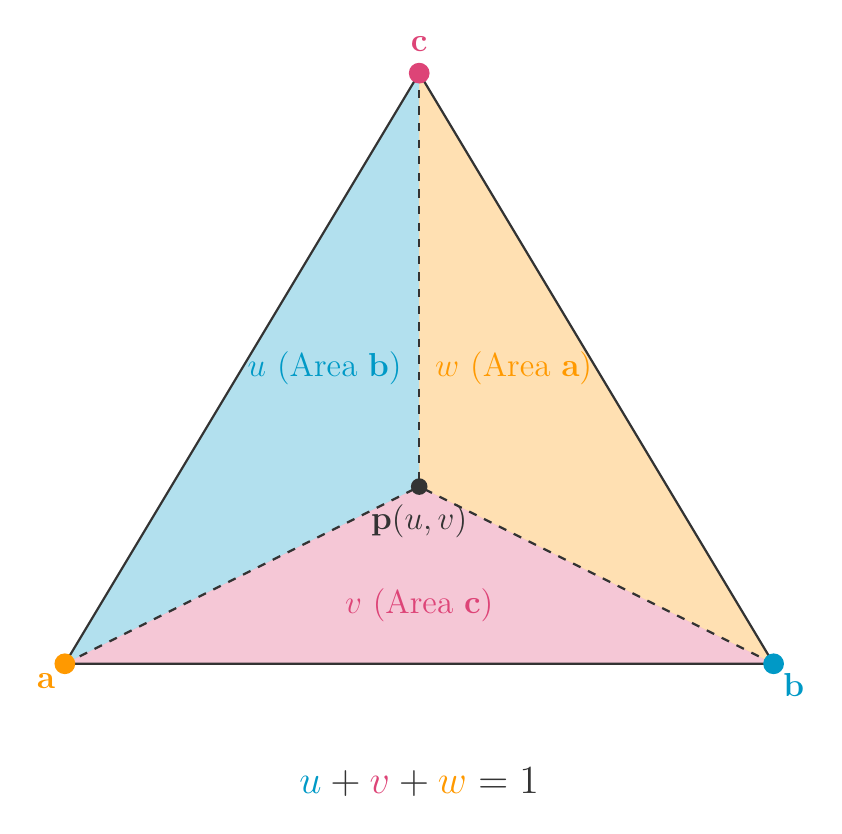
\begin{tikzpicture}[scale=1.5]
    % Triangle Vertices
    \coordinate (A) at (1, 1);
    \coordinate (B) at (7, 1);
    \coordinate (C) at (4, 6);
    % Point P inside
    \coordinate (P) at (4, 2.5);

    % Sub-triangles filled with semi-transparent colors
    \fill[Acol, opacity=0.3] (B) -- (C) -- (P) -- cycle; % Area opposite to A
    \fill[Bcol, opacity=0.3] (A) -- (C) -- (P) -- cycle; % Area opposite to B
    \fill[Ctri, opacity=0.3] (A) -- (B) -- (P) -- cycle; % Area opposite to C

    % Outline
    \draw[thick, Textcol] (A) -- (B) -- (C) -- cycle;

    % Internal dashed lines to P
    \draw[dashed, thick, Textcol] (A) -- (P);
    \draw[dashed, thick, Textcol] (B) -- (P);
    \draw[dashed, thick, Textcol] (C) -- (P);

    % Vertices
    \fill[Acol] (A) circle (2.5pt) node[below left, font=\large] {$\mathbf{a}$};
    \fill[Bcol] (B) circle (2.5pt) node[below right, font=\large] {$\mathbf{b}$};
    \fill[Ctri] (C) circle (2.5pt) node[above, font=\large] at (4.0, 6.1) {$\mathbf{c}$};

    % Point P
    \fill[Textcol] (P) circle (2pt) node[below=3pt, font=\large] {$\mathbf{p}(u,v)$};

    % Area Labels
    \node[Acol, font=\large] at (4.8, 3.5) {$w$ (Area $\mathbf{a}$)};
    \node[Bcol, font=\large] at (3.2, 3.5) {$u$ (Area $\mathbf{b}$)};
    \node[Ctri, font=\large] at (4, 1.5) {$v$ (Area $\mathbf{c}$)};

    % Equation at the bottom (color-coded)
    \node[Textcol, font=\Large] at (4, 0) {$\textcolor{Bcol}{u} + \textcolor{Ctri}{v} + \textcolor{Acol}{w} = 1$};
\end{tikzpicture}

\end{document}